This chapter outlines the methodological framework employed in the design, development, and evaluation of the \textit{Centralized Ultrasonic Sensor-Based Traffic Management System for Speed Limit Violation Detection and Automated Penalty Enforcement}. The primary objective of this section is to detail the structured and systematic approach used to transform conceptual goals into a functional prototype that accurately detects speed violations and autonomously enforces penalties.

The methodology integrates multiple engineering domains—including ultrasonic signal acquisition, embedded system integration, digital signal processing, and network communication protocols—into a cohesive workflow. Instead of immediately presenting technical implementations, this chapter begins with a high-level overview of the system architecture and proceeds to explain the processing pipeline used to estimate vehicle speed based on time-of-flight (ToF) measurements from ultrasonic sensors.

Subsequent sections elaborate on hardware selection (including Arduino and Raspberry Pi boards), software implementation for real-time speed calculation and license plate recognition, system calibration, and testing procedures. The system uses a threshold-based activation mechanism: when the ultrasonic sensor detects a speed violation, the Raspberry Pi triggers image processing and performs license plate recognition.

\section{Overview of Methodological Approach}
\label{sec:methodology-overview}

The methodological approach adopted in this study follows a modular and sequential framework, where each subsystem contributes to the overall functionality of the centralized ultrasonic-based traffic management system. The process begins with vehicle detection and speed estimation using a single ultrasonic sensor. The system measures the time-of-flight (ToF) of reflected ultrasonic pulses to estimate the distance of a moving vehicle at two successive timestamps. By calculating the change in distance over time, the vehicle's speed is computed in real time.

In parallel, a camera module continuously captures images of approaching vehicles. However, image processing procedures—including license plate recognition—are only initiated if the computed speed exceeds a predefined threshold. This conditional processing reduces computational load on the Raspberry Pi and conserves system resources.

Once the vehicle’s license plate number is extracted, relevant metadata—including speed, timestamp, and license plate number—is appended into a locally hosted SQLite database. This database maintains a historical log of all violations and links repeated offenses to the same vehicle. Upon confirmation of a violation, the system automatically sends an email notification containing the violation details and associated penalty.

This structured methodology ensures a streamlined and resource-efficient integration between sensing, decision-making, and enforcement, making the system scalable, cost-effective, and practical for real-world traffic monitoring applications.


\section{Limitations and Assumptions}

The methodology assumes a direct line-of-sight between the sensor and the target vehicle. It is optimized for single-vehicle detection and may exhibit limitations when multiple moving targets are present simultaneously. Environmental factors such as extreme weather or reflective clutter may affect accuracy.



\section{System Architecture}
\label{sec:system-architecture}
The architecture of the Centralized Ultrasonic-Based Traffic Management System for Speed Limit Violation Detection and Automated Penalty Enforcement is designed as a standalone embedded proof-of-concept solution that integrates sensing, processing, and enforcement functionalities. The system comprises two main processing units: an Arduino microcontroller and a Raspberry Pi single-board computer, each assigned specific roles to ensure efficient operation.

The Arduino interfaces with a single ultrasonic sensor to measure the time-of-flight (ToF) of acoustic pulses reflected by passing vehicles, estimating the distance at two successive time intervals. Using these measurements, the Arduino calculates the vehicle’s speed in real time. This speed data is then transmitted to the Raspberry Pi through GPIO communication.

Meanwhile, the Raspberry Pi continuously captures road images using a Pi Camera Module. However, image processing—including license plate recognition via OpenCV and EasyOCR—is initiated only when the speed received from the Arduino exceeds the predefined speed limit. This conditional approach minimizes unnecessary computation, thereby optimizing system performance.

Once a speeding violation is detected, the Raspberry Pi performs license plate number (LPN) extraction. Subsequently, the extracted LPN is used to filter driver information from a hardcoded lookup table containing details such as the driver’s name, email address, and status. The system then records the violation—including speed, timestamp, and license plate number—in a locally hosted SQLite database.

Finally, an automated email notification is generated and sent to the offending driver. This email contains details of the violation, including the fine amount and the reason for the penalty. The violation record is updated accordingly to reflect the enforcement action.

This modular design ensures clear separation of low-level sensing tasks and high-level processing and decision-making, enabling scalable integration with centralized traffic management systems or cloud-based analytics platforms in future developments.
.
\begin{figure}[htbp]
    \centering
    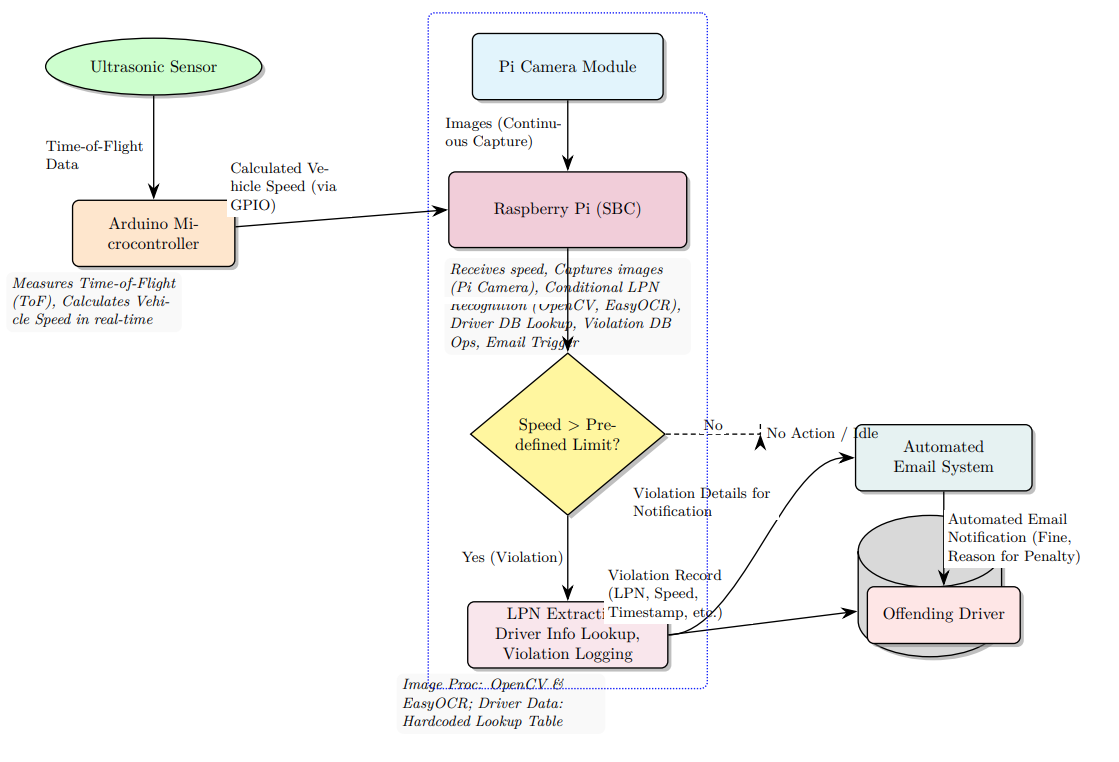
\includegraphics[width=1.0\textwidth]{figures/system_architecture_diagram.png}
    \caption{System architecture diagram}
    \label{fig:system_arch}
\end{figure}

\section{Ultrasonic-Based Speed Detection Module}
\label{sec:ultrasonic-speed-detection}

\subsection*{Principle of Ultrasonic Time-of-Flight Ranging}
Ultrasonic range measurement relies on the time-of-flight (ToF) of high-frequency acoustic pulses between an emitter and a reflecting surface. The sensor emits a short burst of ultrasonic sound (typically around 40~kHz), which propagates through the air at the local speed of sound $c$. When the pulse encounters a vehicle, it reflects back to the sensor's receiver. By measuring the round-trip time $t$, the distance $d$ to the vehicle is computed as:


\begin{equation}
  d = \frac{c \times t}{2}
  \label{eq:tof_distance}
\end{equation}

\begin{figure}[htbp]
  \centering
  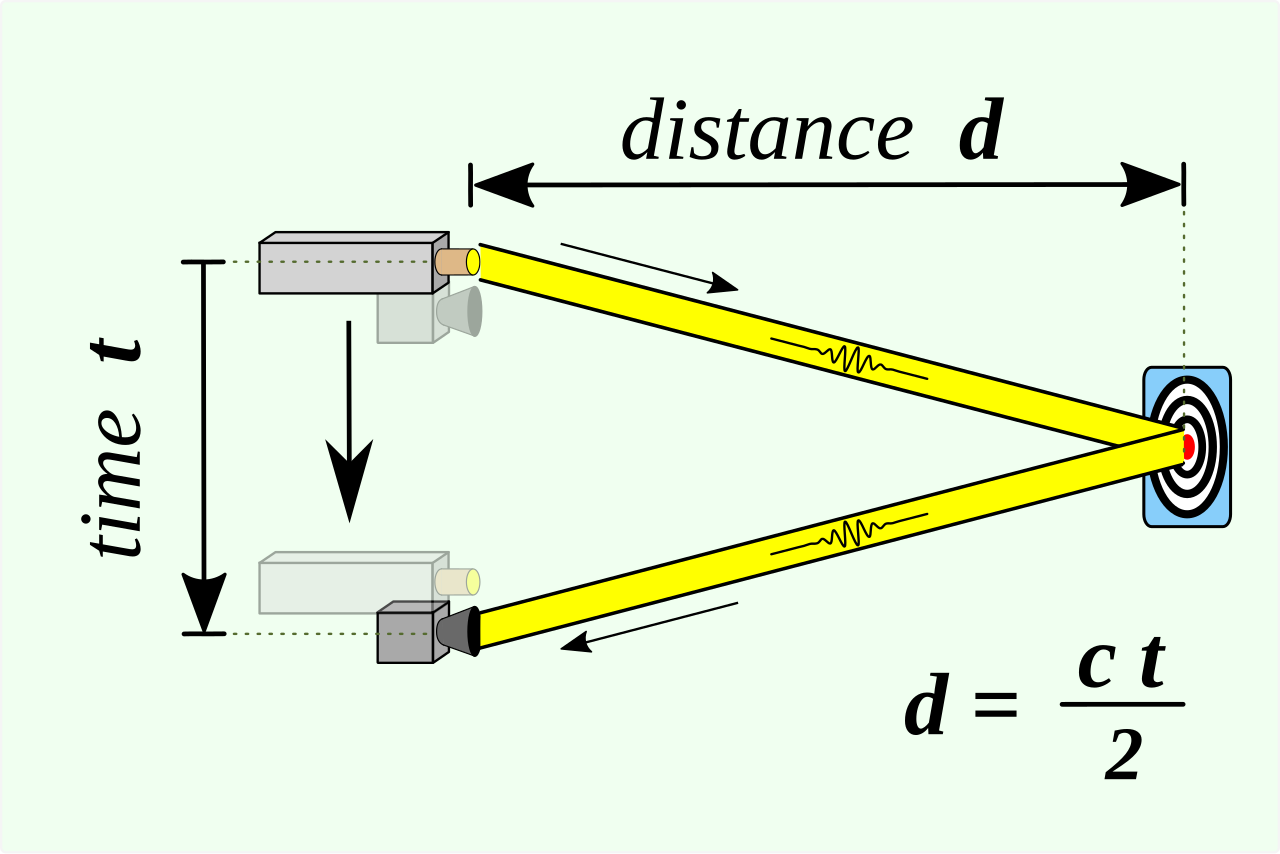
\includegraphics[width=0.8 \linewidth]{figures/ultrasonic.png}
    \caption{HC-SR04 Ultrasonic Sensor for Distance and Speed Estimation}
  \label{fig:ultrasonic-sensor}
\end{figure}


Because the speed of sound in dry air at 20~°C is approximately 343~m/s—and varies by roughly 0.6~m/s for each °C change—many implementations include temperature compensation to maintain accuracy in different environmental conditions.\cite{smith2020ultrasonic}

To determine vehicle speed, the system takes two distance measurements $d_1$ and $d_2$ at times $t_1$ and $t_2$, respectively. Assuming straight-line motion and negligible acceleration between samples, the average speed $v$ over the interval $\Delta t = t_2 - t_1$ is:

\begin{equation}
  v = \frac{d_1 - d_2}{\Delta t}
  \label{eq:speed_estimation}
\end{equation}
In practice, the Arduino microcontroller triggers the ultrasonic sensor at fixed intervals (every 50~ms), computes $d$ for each pulse, and then calculates $v$ in real time. This approach yields a continuous stream of speed data without requiring Doppler processing hardware.\cite{johnson2019measuring}

\subsection*{Implementation of HC-SR04 Ultrasonic Sensor}
The HC-SR04 ultrasonic ranging module is widely used for short-range distance measurement in embedded systems due to its affordability, reliability, and ease of interfacing with microcontrollers. It operates on the principle of ultrasonic time-of-flight (ToF) and provides digital timing signals corresponding to the round-trip duration of an ultrasonic pulse.

\subsubsection{Sensor Architecture and Signal Timing}
The HC-SR04 integrates an ultrasonic transmitter and receiver into a single compact unit. The measurement cycle begins when the microcontroller sends a 10~µs HIGH pulse to the sensor's \texttt{TRIG} (trigger) pin. This pulse initiates the emission of an 8-cycle burst of 40~kHz ultrasonic waves from the transmitter. Simultaneously, the sensor begins timing the echo signal.

These waves propagate through the air until they encounter a reflective object (e.g., a vehicle). The reflected wave is then captured by the receiver. Upon detecting the echo, the sensor pulls the \texttt{ECHO} pin HIGH for a duration proportional to the total round-trip time $t$ of the pulse.

The host microcontroller reads this duration $t$ in microseconds (µs), and the distance $d$ to the target is calculated using:
\begin{equation}
  d = \frac{c \times t}{2}
  \label{eq:hc_distance_eq}
\end{equation}
where $c$ is the speed of sound in air (typically 343~m/s at 20~\textdegree C), and the division by 2 accounts for the round-trip nature of the signal. In practical terms, this is often converted to a simplified empirical formula in centimeters:
\begin{equation}
  d~[\text{cm}] = \frac{t~[\mu s]}{58}
  \label{eq:empirical_cm}
\end{equation}
This approximation assumes $c = 343$~m/s and simplifies real-time processing on microcontrollers like Arduino.

\subsubsection{Speed Estimation Methodology}
To measure the speed of a moving vehicle, the sensor records two consecutive distance readings $d_1$ and $d_2$ at timestamps $t_1$ and $t_2$, respectively. Assuming uniform linear motion between these two readings, the average speed $v$ can be calculated as:
\begin{equation}
  v = \frac{d_1 - d_2}{t_2 - t_1}
  \label{eq:hc_speed}
\end{equation}
The sensor is typically polled at fixed intervals $\Delta t = t_2 - t_1$ (e.g., 50~ms), determined by the microcontroller’s timing logic. Using this periodic sampling, the Arduino continuously computes the instantaneous speed of the object in real-time. A positive value of $v$ indicates motion toward the sensor, while a negative value implies recession.

\subsubsection{Arduino-Based Implementation}
The following high-level steps summarize the software implementation of the HC-SR04 with an Arduino:
\begin{enumerate}
  \item \textit{Trigger Emission}: Set the \texttt{TRIG} pin HIGH for 10~µs to generate an 8-cycle burst.
  \item \textit{Echo Measurement}: Wait for the \texttt{ECHO} pin to go HIGH, and measure the duration $t$ it remains HIGH.
  \item \textit{Distance Calculation}: Convert the duration $t$ to distance using Equation~\ref{eq:empirical_cm}.
  \item \textit{Speed Estimation}: Store successive distance measurements and apply Equation~\ref{eq:hc_speed}.
\end{enumerate}

\subsubsection{Measurement Range and Accuracy}
The HC-SR04 is rated for distances between 2~cm and 400~cm, with typical resolution around ±3~mm under ideal conditions. However, factors such as temperature, humidity, and reflective surface characteristics can introduce errors. Temperature compensation is thus crucial for applications requiring high accuracy. Since the speed of sound $c$ varies approximately by 0.6~m/s per 1~\textdegree C change in air temperature, some implementations use a temperature sensor to adjust $c$ in Equation~\ref{eq:hc_distance_eq}.
\begin{equation}
  c = 331.4 + 0.6T
  \label{eq:temp_compensation}
\end{equation}
where $T$ is the ambient temperature in degrees Celsius.

\subsubsection*{System Integration and Real-Time Considerations}
In the implemented vehicle speed detection system, the HC-SR04 ultrasonic sensor is mounted at a fixed roadside position with an unobstructed line of sight toward approaching vehicles. The Arduino microcontroller manages the emission and reception of ultrasonic pulses at regular intervals, allowing it to compute the speed of passing vehicles in real time. Once a speed value is calculated, it is transmitted to the Raspberry Pi through the serial communication interface. Upon receiving this data, the Raspberry Pi evaluates whether the measured speed exceeds a predefined speed limit. If so, it initiates the image capture process and proceeds with license plate recognition to identify the violating vehicle.

\begin{figure}[htbp]
    \centering
    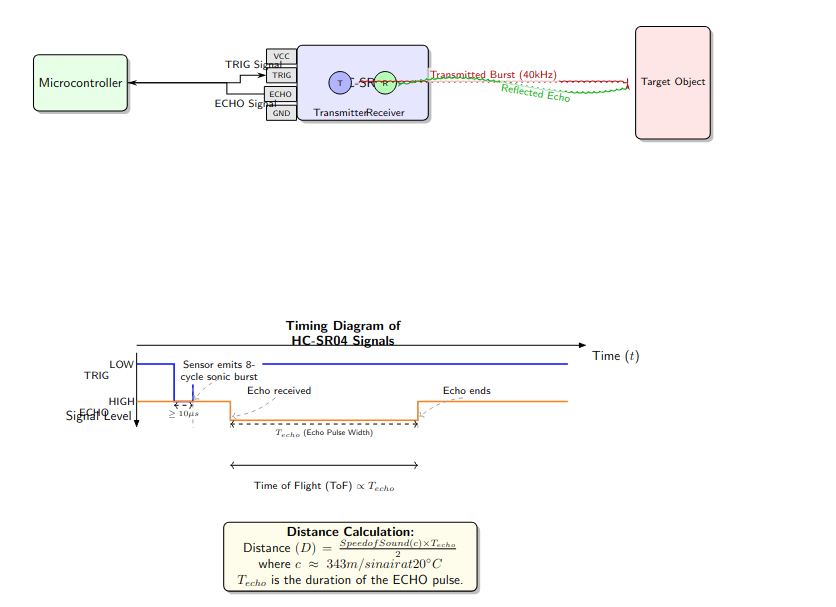
\includegraphics[width=1.0\textwidth]{figures/HC-SR04.png}
    \caption{HC-SR04 Working Principle (Detailed)}
    \label{fig:hc-sr04-detailed}
\end{figure}

\newpage
\subsection*{Advantages and Limitations}
Ultrasonic ToF-based speed detection offers:
\begin{itemize}
  \item {Simplicity and low cost}: Minimal signal processing and inexpensive hardware.
  \item {Robustness}: Works in low-light and varied weather conditions where optical sensors may fail.
\end{itemize}
However, it is subject to:
\begin{itemize}
  \item {Environmental sensitivity}: Variations in temperature, humidity, and wind can affect the speed of sound and introduce errors if uncompensated.
  \item {Beam divergence}: Wide acoustic beams may reflect off unintended surfaces (e.g., ground or nearby structures), requiring careful sensor placement and signal filtering.
\end{itemize}
By understanding these trade-offs, the ultrasonic module can provide reliable speed measurements for triggering downstream license-plate recognition and penalty enforcement in an embedded traffic management system.



\section{Image Capture and License Plate Recognition (LPR)}

This section details the technical methodology employed for the development of the License Plate Recognition (LPR) system, encompassing the hardware setup for image acquisition and the intricate software pipeline for license plate localization and character recognition.

\subsection{Image Acquisition Subsystem}
\label{subsec:image_acquisition}

The image acquisition subsystem is responsible for capturing high-resolution visual data of vehicles, which serves as the primary input for the LPR process.

\subsubsection{Hardware Components}
\label{subsubsec:hardware}

\begin{itemize}
    \item \textbf{Raspberry Pi:} The \textbf{Raspberry Pi 3 Model B+} (with 1GB LPDDR2 SDRAM) serves as the embedded computing platform. Its Broadcom BCM2837B0, Cortex-A53 (ARMv8) 64-bit SoC operating at 1.4GHz provides sufficient processing power for on-device image processing tasks, minimizing latency. The integrated General-Purpose Input/Output (GPIO) pins facilitate direct interfacing with the camera module.
    \item \textbf{Raspberry Pi Camera Module:} Image capture is performed by the \textbf{Raspberry Pi Camera Module V2}. This 8-megapixel camera, featuring a Sony IMX219 sensor, is connected via the dedicated CSI (Camera Serial Interface) port, ensuring high-bandwidth data transfer. The camera is configured to capture still images at a resolution of 720*640 pixels, which provides ample detail for subsequent license plate analysis.

\end{itemize}

\subsubsection{Image Capture Mechanism}
\label{subsubsec:capture_mechanism}

In our implementation, the Raspberry Pi continuously captures still images at fixed time intervals, rather than waiting for an external trigger. Specifically, the camera module is programmed to acquire a high-resolution frame (720×1640 px JPEG) every 100 ms (10 Hz) using a simple loop and the Picamera2 API. Each capture is immediately timestamped and stored—in a directory structured by date and time—to guarantee chronological ordering and ease of retrieval. As soon as an image is written to disk, it is pushed into the OpenCV/EasyOCR processing pipeline for license‐plate localization and character recognition. By decoupling acquisition from motion detection, this periodic sampling approach ensures that no vehicle passing through the sensing zone goes unrecorded, while still bounding CPU and I/O usage by limiting the frame rate to a level that our hardware can sustain in real time..

\subsection*{License Plate Recognition Algorithm}
\label{subsec:lpr_algorithm}

The core of the LPR system is a multi-stage software algorithm implemented primarily in Python, leveraging the \code{OpenCV} and \code{EasyOCR} libraries. The algorithm sequentially processes the captured image to localize the license plate and subsequently recognize its alphanumeric characters.

\begin{figure}[htbp]
    \centering
    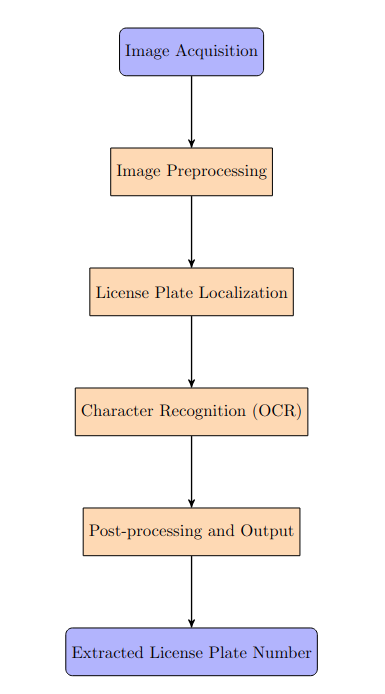
\includegraphics[width=0.95 \textwidth]{figures/LPR.png}
    \caption{ Flowchart of the License Plate Recognition (LPR) Algorithm}
    \label{fig:lpr-flow-chart}
\end{figure}


\subsubsection{Image Preprocessing}
\label{subsubsec:preprocessing}

The initial step involves transforming the raw captured image into a format suitable for robust feature extraction and analysis.

\begin{itemize}
    \item \textbf{Grayscale Conversion:} The 3-channel RGB image is converted to a single-channel grayscale image using \code{cv2.cvtColor(image, cv2.COLOR\_BGR2GRAY)}. This reduces computational complexity by focusing solely on intensity variations, which are critical for edge detection.
    \item \textbf{Noise Reduction:} A \textbf{Gaussian blur} filter is applied to the grayscale image using \code{cv2.GaussianBlur(image, (5, 5), 0)}. This operation smooths the image, reducing high-frequency noise and mitigating the impact of minor imperfections or illumination variations, thereby preventing spurious edges in subsequent steps.
    \item \textbf{Contrast Enhancement:} To improve the distinction between license plate characters and their background, especially under non-uniform lighting, Adaptive Histogram Equalization (AHE), specifically \textbf{Contrast Limited Adaptive Histogram Equalization (CLAHE)}, is applied. This is implemented via \code{cv2.createCLAHE(clipLimit=2.0, tileGridSize=(8,8))} followed by \code{apply()}. CLAHE enhances local contrast without over-amplifying noise in homogeneous regions.
\end{itemize}

\subsubsection{License Plate Localization}
\label{subsubsec:localization}

This stage aims to accurately identify and extract the rectangular region containing the license plate from the preprocessed image.

\begin{itemize}
    \item \textbf{Edge Detection:} The \textbf{Canny edge detector} is applied to the contrast-enhanced grayscale image using \code{cv2.Canny(image, 100, 200)}. This algorithm identifies strong intensity gradients, effectively highlighting potential boundaries of objects, including the license plate and its characters. The thresholds (100 and 200) are empirically determined to balance sensitivity and noise suppression.
    \item \textbf{Morphological Operations:} To connect fragmented edges and enhance the rectangular shape of the license plate, a sequence of morphological operations is performed:
    \begin{itemize}
        \item \textbf{Dilation:} \code{cv2.dilate(edges, kernel, iterations=1)} is applied to thicken the edges and close small gaps, using a rectangular kernel.
        \item \textbf{Erosion:} \code{cv2.erode(dilated\_edges, kernel, iterations=1)} is then applied to thin the thickened edges, effectively removing small noise components while preserving the connected larger structures. This `dilate` then `erode` sequence is equivalent to a \textbf{closing} operation, which is effective at closing small holes and connecting nearby features.
    \end{itemize}
    \item \textbf{Contour Detection and Filtering:}
    \begin{itemize}
        \item \textbf{Contour Finding:} Contours (continuous curves joining all continuous points along the boundary, having the same color or intensity) are detected using \code{cv2.findContours(processed\_edges, cv2.RETR\_LIST, cv2.CHAIN\_APPROX\_SIMPLE)}.
        \item \textbf{Contour Approximation:} Each detected contour is approximated to a simpler polygon using \code{cv2.approxPolyDP(contour, epsilon, True)}, where $\epsilon$ is a small fraction of the contour perimeter. This helps in identifying rectangular shapes more robustly.
        \item \textbf{Filtering by Geometric Properties:} Candidate contours are rigorously filtered based on their geometric properties, which are characteristic of standard license plates:
        \begin{itemize}
            \item \textbf{Area:} Contours with an area (\code{cv2.contourArea}) outside a predefined range (e.g., $A_{\text{min}} \le A \le A_{\text{max}}$) are discarded.
            \item \textbf{Aspect Ratio:} The aspect ratio ($AR = \frac{\text{width}}{\text{height}}$) of the bounding rectangle (\code{cv2.boundingRect}) of each contour is calculated. Typical license plates exhibit an aspect ratio within a specific range, e.g., $2.5 \le AR \le 5.0$ for standard single-line plates.
            \item \textbf{Number of Vertices:} Only contours that, after approximation, have exactly four vertices are considered, indicating a rectangular shape.
            \item \textbf{Solidity:} The ratio of the contour area to the area of its convex hull (\code{cv2.contourArea(cv2.convexHull(contour))}) is checked to ensure the contour is solid and not excessively concave.
        \end{itemize}
    \end{itemize}
    \item \textbf{Region of Interest (ROI) Extraction and Perspective Correction:} The contour that best satisfies all filtering criteria is identified as the license plate. Its bounding box coordinates are extracted. If the license plate is captured at an angle, a perspective transformation is applied to rectify the ROI. This involves:
    \begin{itemize}
        \item Identifying four corner points of the detected license plate.
        \item Defining the corresponding desired output points for a rectified, front-parallel view.
        \item Computing the perspective transformation matrix using \code{cv2.getPerspectiveTransform(src\_points, dst\_points)}.
        \item Applying the transformation to the original image using \code{cv2.warpPerspective(image, M, output\_size)} to obtain a normalized, frontal view of the license plate.
    \end{itemize}
\end{itemize}

\subsubsection{Character Recognition (Optical Character Recognition - OCR)}
\label{subsubsec:ocr}

The localized and rectified license plate ROI is then passed to the OCR engine for character extraction.

\begin{itemize}
    \item \textbf{EasyOCR Integration:} The \code{EasyOCR} library is utilized for this stage. It is initialized with the desired language models (e.g., \code{reader = easyocr.Reader(['en'])} for English).
    \item \textbf{Deep Learning Model:} EasyOCR leverages a combination of deep learning architectures:
    \begin{itemize}
        \item \textbf{Convolutional Recurrent Neural Network (CRNN):} This component extracts features from the image. The Convolutional Neural Network (CNN) layers extract spatial features, which are then fed into Recurrent Neural Network (RNN) layers (specifically, Bidirectional LSTMs) to capture sequential dependencies between features, crucial for recognizing characters in a sequence.
        \item \textbf{Connectionist Temporal Classification (CTC):} This is a loss function used to train recurrent neural networks for sequence labeling problems where the alignment between the input and output sequences is unknown. CTC allows EasyOCR to recognize entire character sequences without explicit segmentation of individual characters, making it robust to variations in character spacing and font.
    \end{itemize}
    \item \textbf{Recognition Output:} The \code{reader.readtext(roi\_image)} function processes the license plate ROI and returns a list of detected text boxes, each containing the recognized text, its bounding box, and a confidence score.
\end{itemize}

\subsubsection{Post-processing and Output}
\label{subsubsec:postprocessing}

The raw OCR output undergoes a final stage of refinement to ensure accuracy and adherence to expected license plate formats.

\begin{itemize}
    \item \textbf{Text Concatenation:} If EasyOCR returns multiple text boxes for a single plate (e.g., due to slight gaps), these are concatenated into a single string, respecting their horizontal order.
    \item \textbf{Regular Expression Filtering:} A regular expression is applied to the recognized string to filter out non-alphanumeric characters and enforce specific patterns typical of license plates in the target region (e.g., `$$[A-Z]{2,3}[0-9]{3}[A-Z]{2}$$` for a hypothetical format). This helps in removing noise and standardizing the output.
    \item \textbf{Error Correction Heuristics:} Common OCR errors (e.g., 'O' vs. '0', 'I' vs. '1', 'S' vs. '5', 'B' vs. '8') are addressed using a set of predefined substitution rules or a lookup table based on common character ambiguities and regional license plate patterns. For instance, if a character 'O' is detected in a position typically reserved for numbers, it might be corrected to '0' based on context.
    \item \textbf{Final Output:} The cleaned and validated alphanumeric string representing the license plate number is then output by the system. This output can be stored in a database, displayed on a user interface, or used to trigger further actions (e.g., gate opening).
\end{itemize}




\section{ Violation Handling and Penalty Enforcement}

Once a license-plate has been recognized and the measured speed \(v\) exceeds the predefined threshold \(v_{\mathrm{lim}}\), the system proceeds with storing the violation and notifying the offending driver. This process is implemented via a lightweight SQLite database and an automated email module, as described below.

\subsubsection{Database Schema and Initialization}
A local SQLite database (\texttt{speed\_monitor.db}) is used to persist driver records and violation events. Two tables are created at startup:
\begin{itemize}
  \item \textbf{drivers}: stores  
    \(\{\)\,id, name, license\_plate, email, violation\_count, created\_at\(\}\).  
    Each driver’s license plate is enforced as unique, and \texttt{violation\_count} tracks the cumulative number of recorded offenses.
  \item \textbf{violations}: stores  
    \(\{\)\,id, driver\_id, speed, timestamp, image\_path\(\}\).  
    A foreign key \texttt{driver\_id} references the \texttt{drivers} table.
\end{itemize}
This schema ensures referential integrity and supports efficient querying of both individual driver histories and aggregate statistics.

\subsubsection{Recording a Violation}
When a new violation is detected, the following steps occur:
\begin{enumerate}
  \item \emph{Driver lookup}: retrieve the driver’s record by matching the recognized license plate.  
  \item \emph{Insert violation}: create a new entry in \texttt{violations} with the fields  
    \(\{\)driver\_id, speed, timestamp, image\_path\(\}\).  
  \item \emph{Increment counter}: update the corresponding driver’s \texttt{violation\_count} by \(+1\).
  \item \emph{Commit transaction}: ensure both tables remain consistent by committing the changes atomically.
\end{enumerate}

\subsubsection{Automated Penalty Notification}
Immediately after persisting the violation, the system constructs and sends an email notification to the driver:
\begin{enumerate}
  \item Query the \texttt{drivers} table to obtain the driver’s name and email.
  \item Generate an email containing:
    \begin{itemize}
      \item Date and time of the violation
      \item Recorded speed and applicable speed limit
      \item Amount of the fine and instructions for payment
    \end{itemize}
  \item Dispatch the message via the \texttt{EmailSender} module using SMTP, embedding a link to the stored image for verification.
\end{enumerate}

\subsubsection{Reporting and Analytics}
The database manager also provides methods to retrieve:
\begin{itemize}
  \item The most recent \(N\) violations, with associated driver names and image paths.
  \item The Top \(M\) speeders, ranked by \texttt{violation\_count}, for enforcement prioritization.
  \item A complete list of registered drivers, including their cumulative violation counts and registration timestamps.
\end{itemize}
These queries support both real-time dashboard displays and offline analysis of traffic patterns and repeat offenders.

---

By centralizing all violation data in an embedded SQLite database and linking it to an automated email notification system, the implementation ensures that every detected offense is reliably recorded, the driver is promptly informed, and historical data can be mined for policy or system-tuning purposes.```



